\chapter{Hardware Arkitektur}

\section{Block Definition Diagram}
Vores system kaldet WinePrep, består af en embedded Linux-platform (Devkit-8000), hvor der er mulighed for bruger-input. Linux-platformen er forbundet til en PSoC5 (CY8CKIT-059) via SPI. PSoC platformen anvendes til at styrer positionerings- og åbnings-mekanismerne, som hver består af nogle aktuatorer og sensorer. Positioneringsmekanismen besår af de 3 akser (X,Y,Z) og steppermotorer til at styrer disse, åbningsmekanismen er så fastmonteret herpå, således denne kan positioneres i forhold til vinflasken, så aktuatorer på åbningsmekanismen kan anvendes til at trække proppen.

\begin{figure}[H]
	\centering
	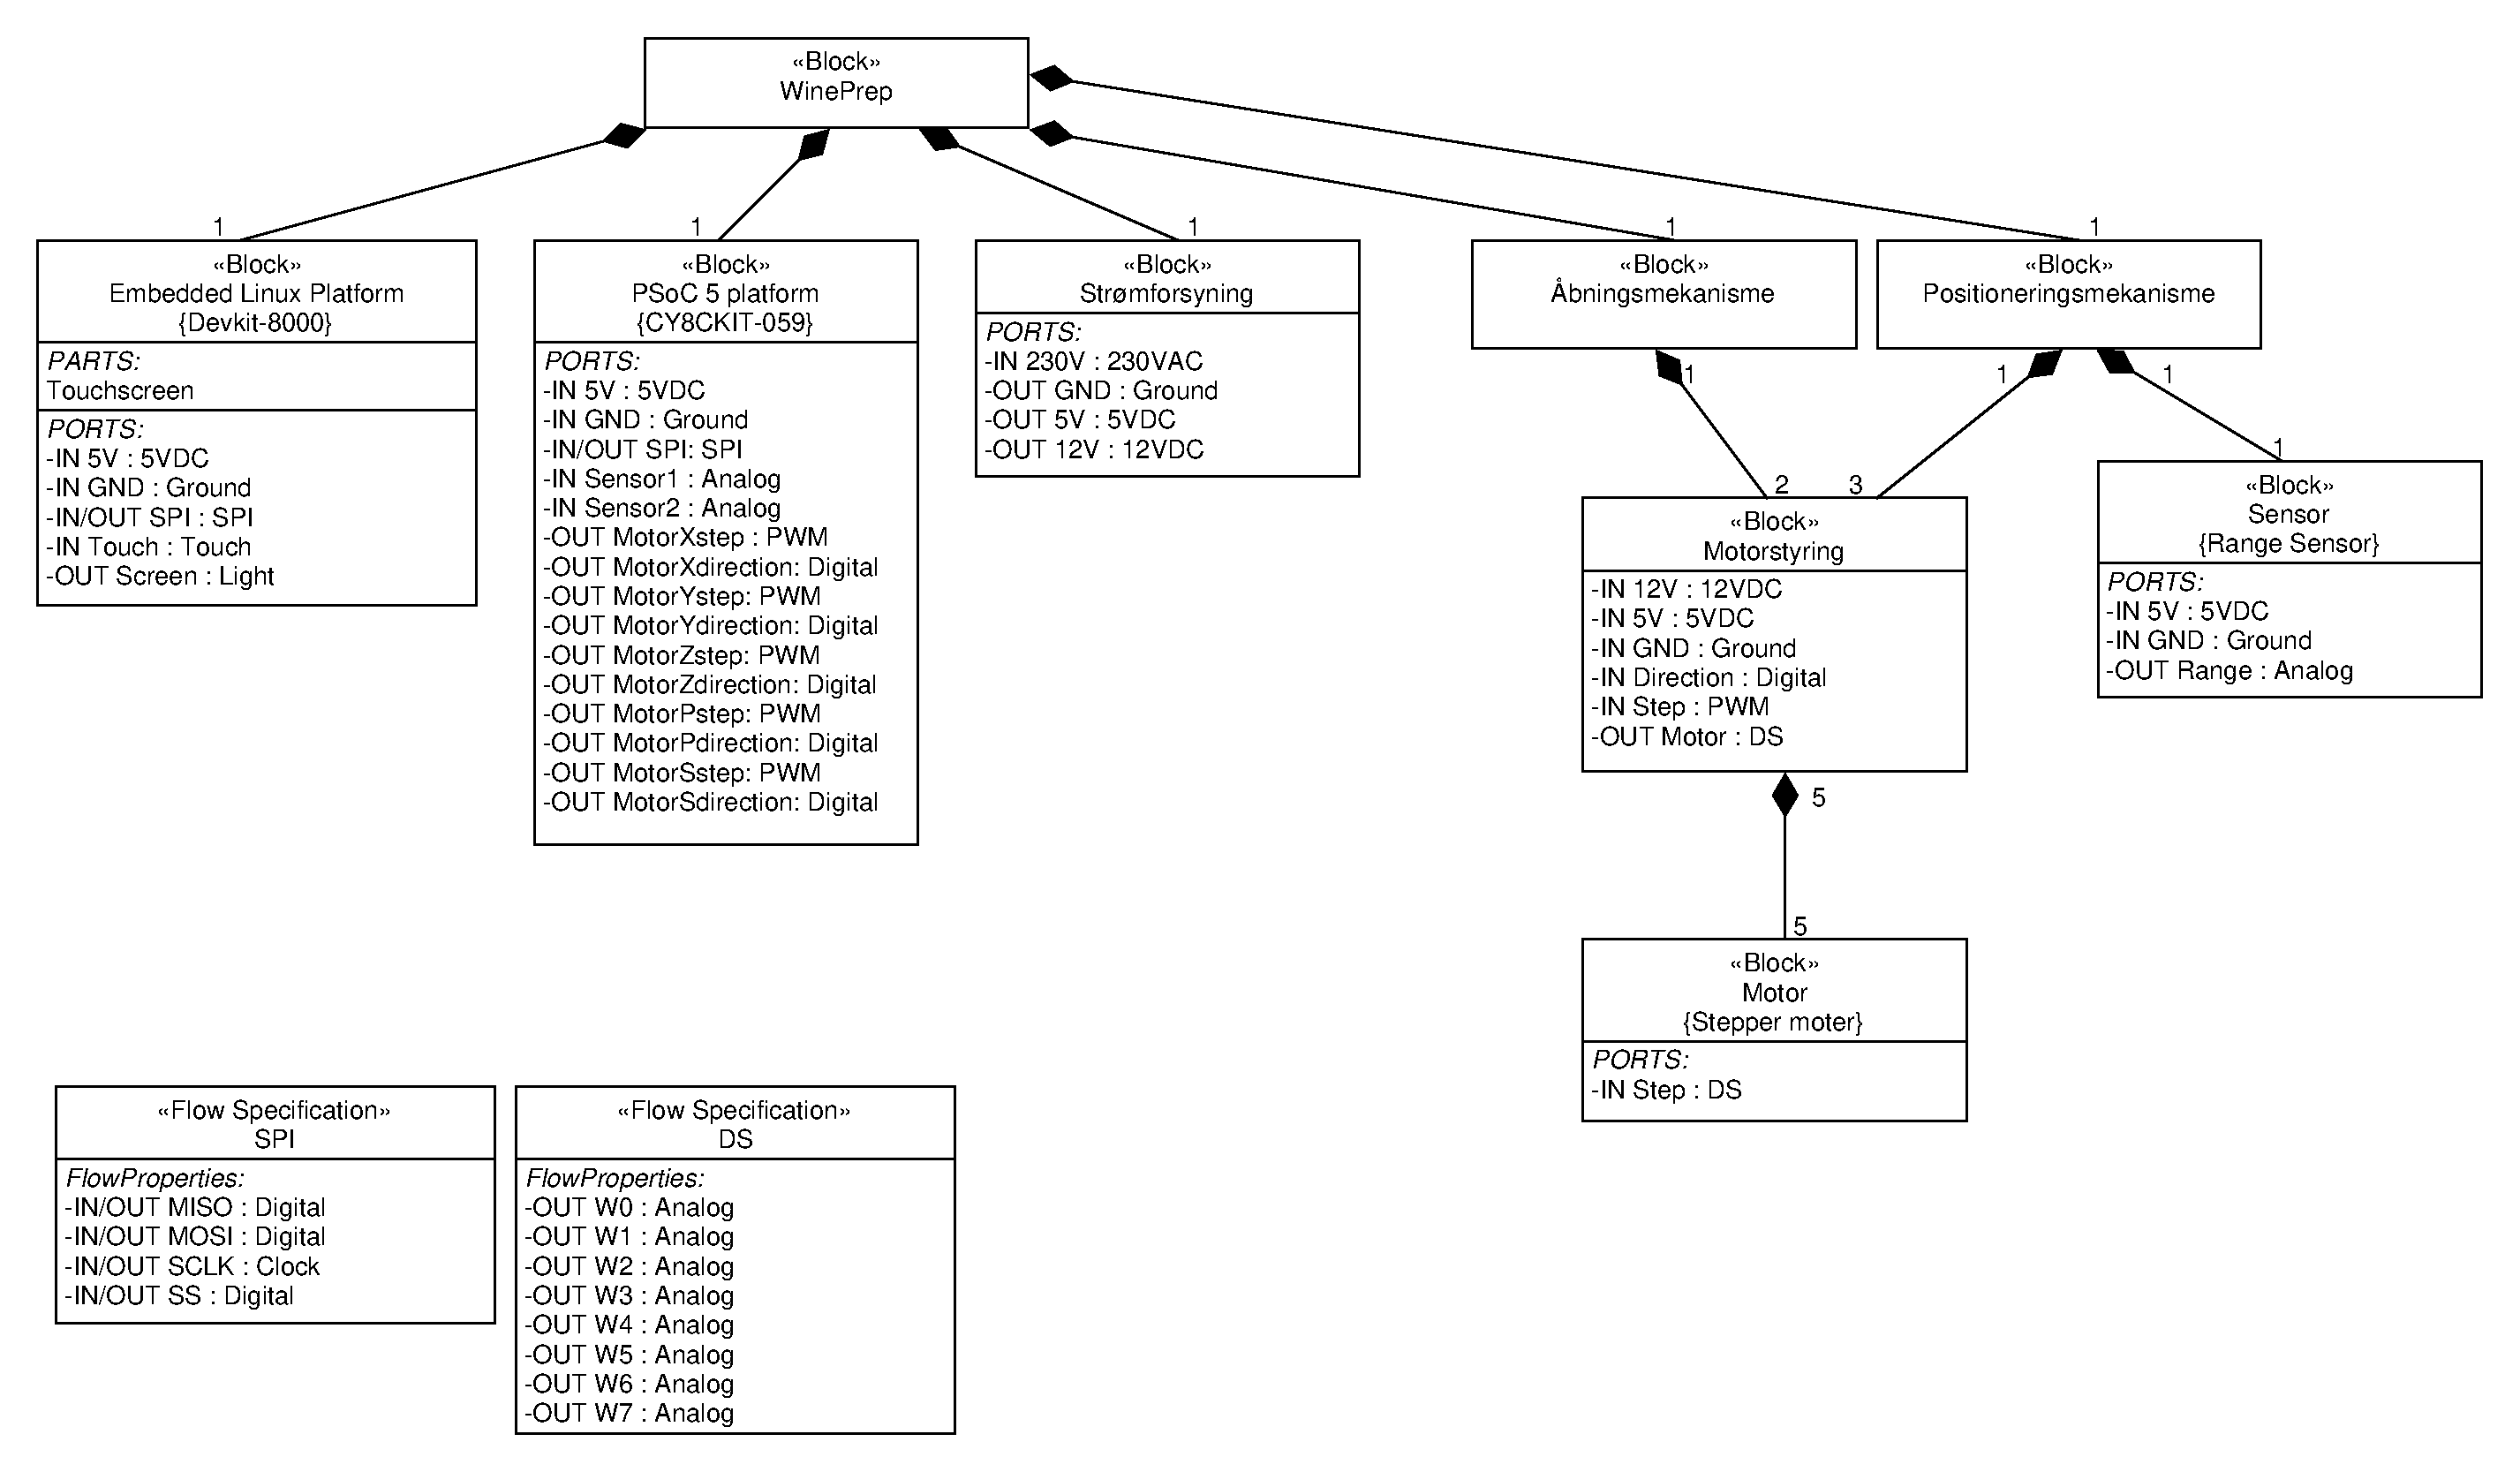
\includegraphics[scale=0.3]{blockdefinitiondiagram}
	\caption{BDD for WinePrep}
	\label{BDD}
\end{figure}

\subsubsection{Blok beskrivelser}
Her følger beskrivelser af de enkelte blokke på vores BDD, se side \pageref{BDD} Figur \ref{BDD}.

\paragraph{WinePrep} blokken er det samlede system der består af underblokkende Embedded Linux Platform, PSoC 5 Platform, Åbningsmekanisme, Positioneringsmekanisme samt strømforsygning.

\paragraph{Embedded Linux Platform} Dette er den blok der håndtere brugerens interaktion med systemet. Blokken består af et Devkit800 med touchskærm. Som styresystem på platformen anvendes der Linux distributionen Ångström. Her fra anvendes der QT til at lave den grafiske brugerflade der vises på touchskærmen til brugeren af systemet. Samtidig kommunikere Embedded Linux Platformen med vores PSoC 5 Platform via SPI standarden.

\paragraph{PSoC 5 Platform} PSoC 5 baseret platform der står for styring af Motor og Sensor blokkene, samt kommunikere med blokken Embedded Linux Platform over SPI.

\paragraph{Strømforsyning} Strømforsyning skal kunne modtage 230V fra dansk stikkontakt, og forsyne systemet med de nødvendige spændinger.

\paragraph{Positioneringsmekanisme} Denne blok indeholder alt hvad vi bruger til at bevæge på vores sensorer når vi scanner flasken, og til at flytte på vores åbningsmekaniske i forhold til flaskens placering. Blokken består dermed af en motorstyrings blok samt en motor blok for hver af de 3 akser.

\paragraph{Åbningsmekanisme} Åbningsmekanismen består af de to motorer som anvendes til at skrue proptrækker-skruen i vinflaskens prop, samt til at trække proppen ud af vinflasken, samt to motorstyrings blokke til disse motorer.

\paragraph{Motorstyring} Motorstyrings blokken består af en CY8CKIT-059, som anvendes til at styrer én motor når der kommer signal fra PSOC5 platforms blokken om dette.

\paragraph{Sensor1} Afstandssensorer til detektering af vinflaskens placering samt størrelse, så åbningsmekanismen ud fra dette kan positioneres korrekt ved hjælp af motorer på X, Y , Z akserne.

\paragraph{Sensor2} Sensor til at detekterer når en akse kommer til et yderpunkt. Anvendes ved at kører aksen ud indtil sensoren aktiveres, og så indstille aksens position til en forud fastlagt værdi.

\paragraph{Motor} Motorblokken er alle de motorer som anvendes i systemet til positionering og prop-træk. Denne blok skal eventuelt opdeles i flere forskellige blokke hvis vi får brug for at anvende andre typer motorer end steppermotorer.

\subsection{Ting der først bliver fast besluttet på senere iterationer/sprints}

Motor Valg er ikke 100\% fastlagt, hvorfor det her i BDD modelleres med stepper motors, og portene er derfor heller ikke 100\% korrekte da dette afhænger af motorstyringen.

Sensor typer og antal ligger kun delvist fast. Der vil være 2 afstandssensorer til detektering af vinflaskens placering, samt 3 sensorer af ikke nærmerer fastlagt type til at detekterer hvis en akse når til et yderpunkt. Afstands sensorer til detektering af vinflaskens position, bliver enten lys baserede eller lydbaserede, der vil give et analog output signal i form af en spænding der afhænger af afstanden. Sensorer til detektering på aksernes yderpunkter overvejes implementeret med en switch, eller eventuelt strain gauge.

\section{Internal Block Diagram}

\begin{figure}[H]
	\centering
%	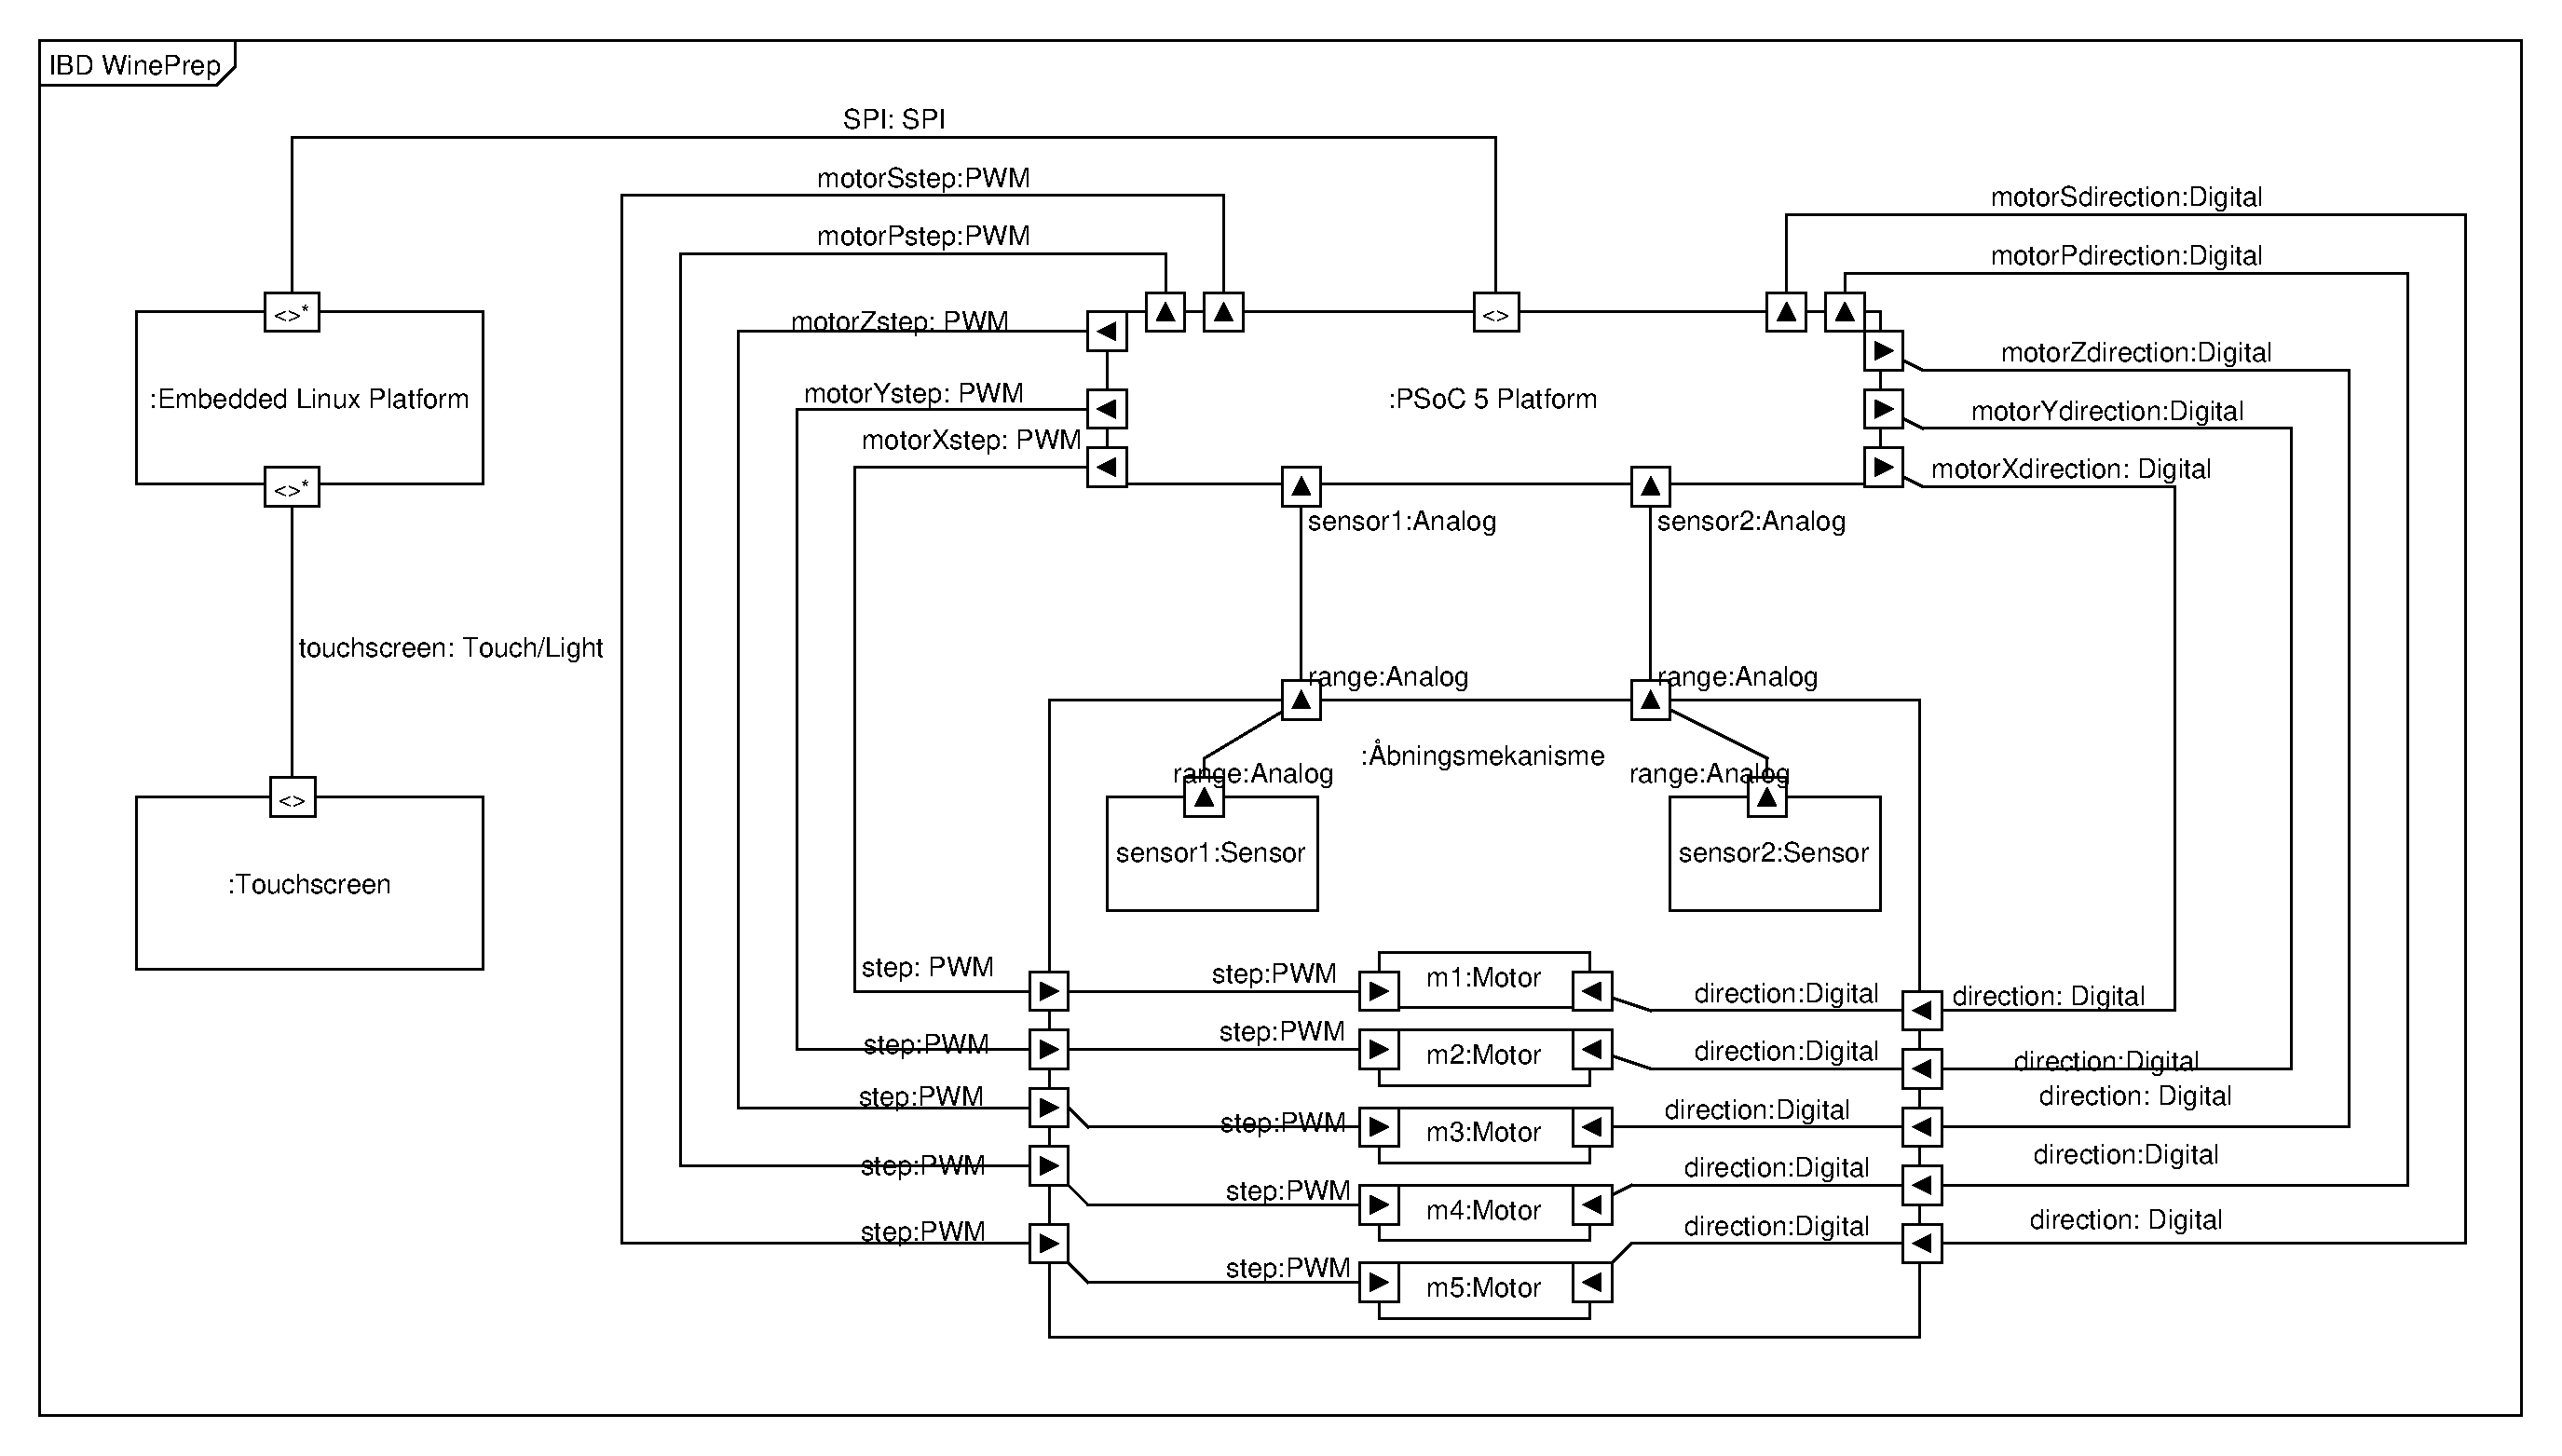
\includegraphics[scale=0.3]{IBDiagram}
	\caption{IBD for WinePrep}
	\label{IBD}
\end{figure}

\subsection{Signal Beskrivelser}

\begin{tabular}{>{\bfseries}p{50pt}  p{110pt}  p{170pt}}
	Signal Type & \textbf{Porte} & \textbf{Beskrivelse} \\
	Digital & MISO, MOSI, SS, MotorXDirection, MotorYDirection, MotorZDirection, MotorSDirection, MotorPDirection & 0-5V firkant signal \\
	Analog & Range, Sensor1, Sensor2 & Analog Spænding mellem 0-5V \\
	Clock & SCLK & Konstant firkantsignal på 0-5V med 50\% dutycycle og fast frekvens \\
	Touch & Touchscreen & kraftpåvirkning af skærmen \\
	Light & Touchscreen & Lys i varierende farver i det synlige spektrum \\
	PWM & Step, MotorXstep, MotorYstep, MotorZstep, MotorSstep, MotorPstep & 0-5V firkant med varierende dutycycle. \\
	SPI & SPI & Serial Peripheral Interface Bus industri standard \\
\end{tabular}